% ─── Slide: Dead zone was NOT hardware-fundamental ────────────────────────────
\begin{frame}{First Key Discovery: Dead Zone Was Not Hardware-Fundamental}
  \begin{columns}[T]
    \begin{column}{0.50\textwidth}
      \begin{block}{Early baseline (branch \texttt{llama-flatquant-adc})}
        \begin{itemize}
          \item $\bypass = 21.6$, $\adcppl = 28.99$
          \item \texttt{dead\_rate} = \worse{81\%}
          \item PACT, penalties, L1 loss $\Rightarrow$ all failed
        \end{itemize}
      \end{block}

      \vspace{0.5em}
      \begin{exampleblock}{Improved baseline (branch \texttt{pact})}
        \begin{itemize}
          \item $\bypass = 10.0$, $\adcppl = 28.86$
          \item \texttt{dead\_rate} = \better{10.3\%}
          \item \textbf{Hardware unchanged.} Only better FlatQuant training
            (\texttt{percentile} calibration vs.\ \texttt{absmax})
        \end{itemize}
      \end{exampleblock}

      \vspace{0.7em}
      \textbf{Implication:}\\
      Dead-zone collapse was a \alert{transform quality problem},\\
      not a fundamental ADC hardware constraint.\\[0.4em]
      Remaining gap $\bypass{=}10 \to \adcppl{=}29$\\
      is \textbf{ADC resolution} (only $\sim$15--30 bins in $\pm\sigma_z$).
    \end{column}
    \begin{column}{0.46\textwidth}
      % plot_deadzone_not_fundamental.pdf
      \iffalse
        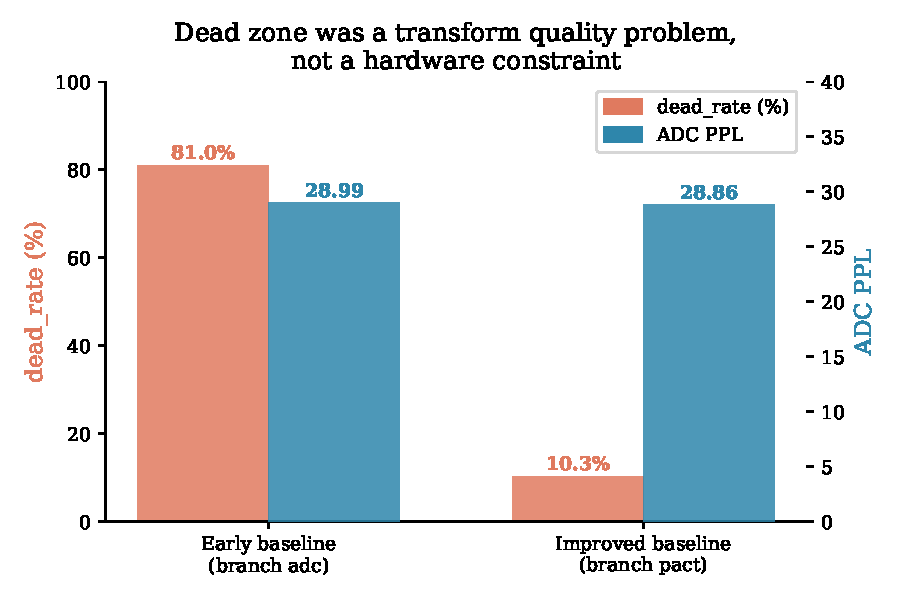
\includegraphics[width=\linewidth]{figs/plot_deadzone_not_fundamental.pdf}
      \else
        \figplaceholder[0.65\textheight]{Grouped bar chart:
          x-axis = \{Early baseline, Improved baseline\},
          two bars per group: dead\_rate (\%) and ADC PPL.
          Values: dead\_rate 81\% $\to$ 10.3\%; ADC PPL 28.99 $\to$ 28.86.
          Note: ADC PPL barely changes despite 8$\times$ dead-rate reduction.}
      \fi
    \end{column}
  \end{columns}
\end{frame}
